\section{O Framework Scrum}

O Scrum é um framework ágil amplamente utilizado no desenvolvimento de software, especialmente em ambientes caracterizados por alta complexidade, incerteza e necessidade de adaptação contínua. Conforme descrito no Scrum Guide \cite{schwaber2020scrum}, o framework estabelece papéis, eventos e artefatos que auxiliam equipes a entregarem valor de forma incremental e iterativa.

O framework Scrum é descrito oficialmente por Schwaber e Sutherland \cite{schwaber2020scrum}.
Ele se baseia nos pilares da transparência, inspeção e adaptação. A transparência garante que todos os aspectos relevantes do processo estejam visíveis aos envolvidos; a inspeção permite a avaliação frequente dos artefatos e do progresso; e a adaptação possibilita ajustes sempre que desvios ou oportunidades de melhoria são identificados.

\subsection{Papéis do Scrum}

O Scrum define três papéis principais: Product Owner, Scrum Master e Time de Desenvolvimento. O Product Owner é responsável por maximizar o valor do produto, gerenciando e priorizando o Product Backlog de acordo com as necessidades dos stakeholders. O Scrum Master atua como facilitador, garantindo que o framework Scrum seja compreendido e aplicado corretamente, além de remover impedimentos que possam impactar o progresso da equipe. Já o Time de Desenvolvimento é composto por profissionais multidisciplinares responsáveis por transformar os itens do backlog em incrementos de produto potencialmente entregáveis.

\subsection{Eventos do Scrum}

Os eventos do Scrum são estruturados para criar regularidade e minimizar a necessidade de reuniões não planejadas. O principal evento é a Sprint, um período de tempo fixo, geralmente entre duas e quatro semanas, no qual um incremento do produto é desenvolvido. A Sprint é composta por eventos como o Sprint Planning, no qual o trabalho é planejado; a Daily Scrum, reunião diária de alinhamento; a Sprint Review, momento de inspeção do incremento; e a Sprint Retrospective, dedicada à reflexão e melhoria contínua do processo.

\subsection{Artefatos do Scrum}

Os principais artefatos do Scrum incluem o Product Backlog, o Sprint Backlog e o Incremento. O Product Backlog é uma lista priorizada de funcionalidades, melhorias e correções necessárias ao produto. O Sprint Backlog representa o conjunto de itens selecionados para a Sprint corrente, juntamente com um plano para sua entrega. O Incremento é a soma de todos os itens concluídos durante a Sprint, atendendo à definição de pronto estabelecida pela equipe.

A adoção do Scrum promove maior previsibilidade, colaboração e capacidade de resposta às mudanças, tornando-o especialmente adequado para projetos de software em contextos dinâmicos e complexos.


A Figura~\ref{fig:ciclo-scrum} ilustra o ciclo do framework Scrum, evidenciando a natureza iterativa e incremental do processo.


\begin{figure}[H]
\centering
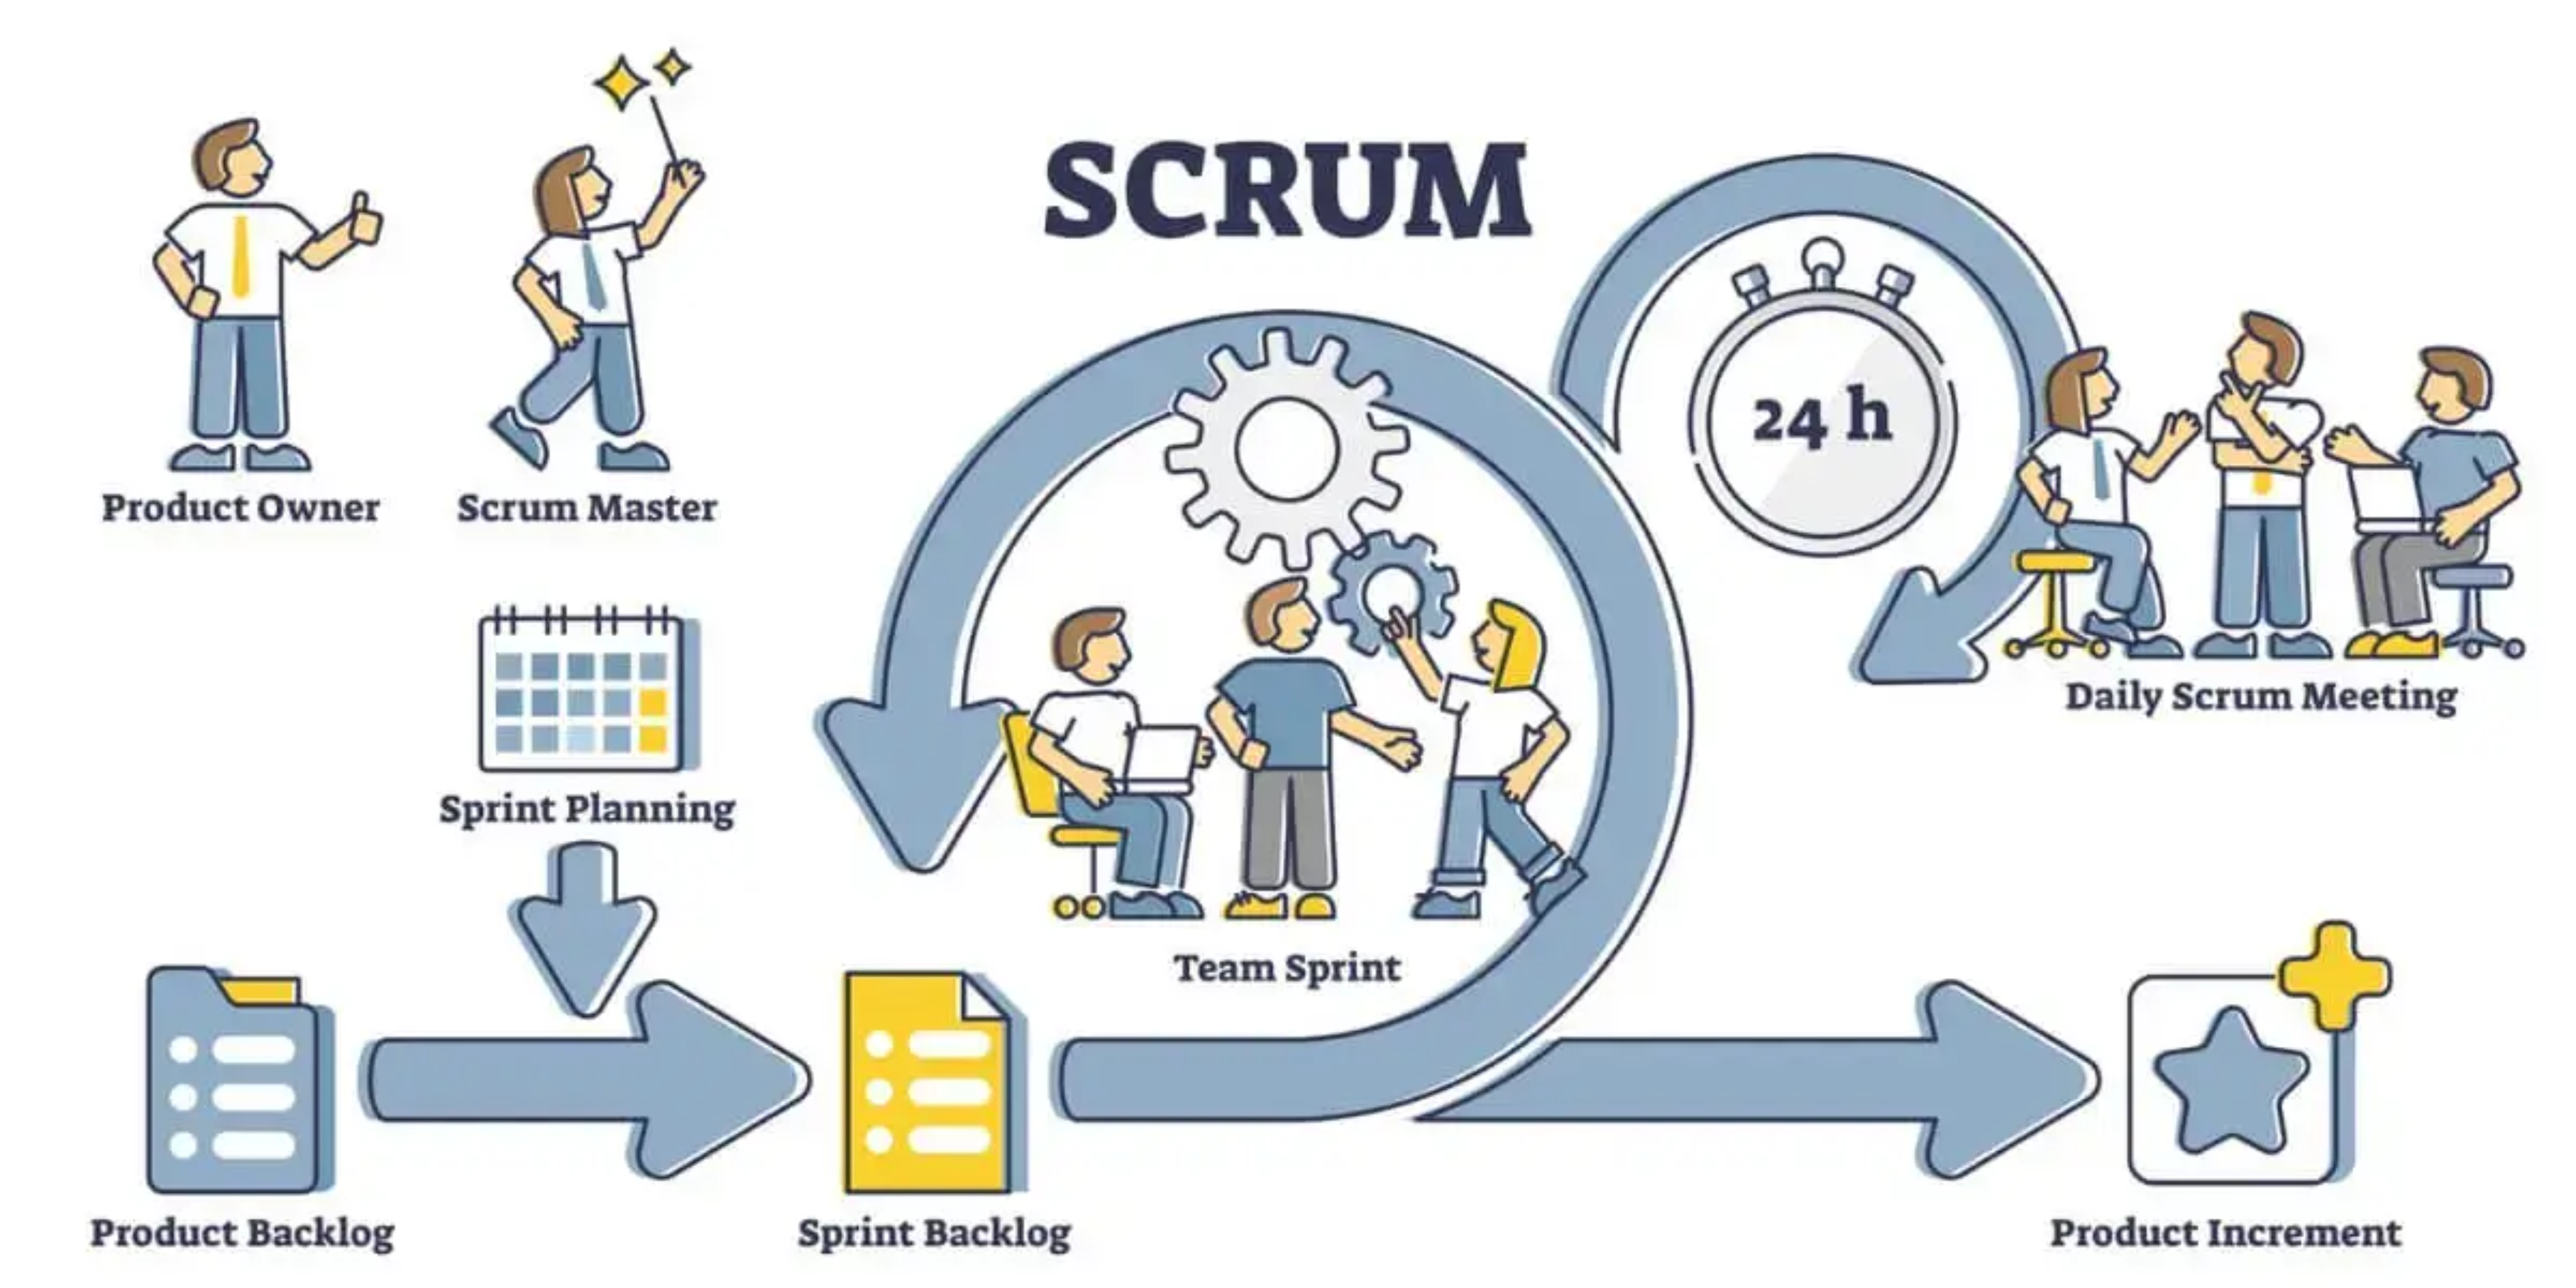
\includegraphics[width=0.75\textwidth]{figuras/scrum-ciclo}
\caption{Benefícios das Metodologias Ágeis}
\label{fig:ciclo-scrum}
\end{figure}
